% $Id: thesis.tex,v 1.60 2010/04/13 11:12:30 dvd Exp $

\documentclass{article}

\usepackage{setspace,geometry}
\usepackage{framed}
\usepackage{graphicx}

\geometry{bindingoffset=0.4in,margin=1.2in}
\onehalfspacing

\author {}

\title{Y5 Report: Optimization Toolkit}

\begin{document}
\maketitle

\section{Rational Value~of~Information Estimation for
  Measurement~Selection}

The optimization algorithms used in the UNCERTIMA Toolkit rely on
computing the value of information of search actions. In general,
computation of value of information, even under the commonly used
simplifying myopic assumption, involves multidimensional integration
of a general function. For some problems, the integral can be computed
efficiently; but when the utility function is computationally
intensive or when a non-myopic estimate is used, the time required to
compute the value of information can be significant and must be taken
into account while computing the value of information. An extended
version of the greedy optimization algorithm has been developed and
implemented in the toolkit.

The rational recomputing algorithm decides when to recompute the value
of information of each of the measurements based on the principles of
limited rationality. The search tool allows to choose either the basic
or the rational recomputing version of the algorithms implemented in
the tool. When a rational recomputing algorithm is chosen, an
additional parameter---the VOI recomputation cost---must be
provided. By varying the parameter, the user can control the overhead
caused by VOI recomputation on the search runtime. Theoretical
analysis and empirical evaluation of the extended algorithm are
provided in the attached paper (file {\tt raticomp.pdf}).

\section{Optimizing Parameters of Expert Rules}
\label{sec:tuning-rules}

Orbotech provided an example of expert rules used for identifying a
particular defect, along with a set of 390 samples for
experimenting. The expert rules are parameterized by 10
parameters. While reasonable values of the parameters can be guessed
by the expert, the performance of the expert rules can be improved by
finding the best values of the parameters for the given training set.

The VOI-based search algorithms work best when the measurements (or
trials) are expensive, and the search space is relatively small. These
two conditions allow to estimate value of information of a trial for
each combination of parameters, and to perform the most promising
trial. However, in the case of tuning expert rules parameters on a
relatively small training test, the situation is just opposite: the
search space is huge, but a single trial is very cheap.

Due to a particular shape of the expert rules, some
parameters are responsible for breaking the samples into big groups,
and the rest are used for fine adjustments of the classification
within the group. Splitting the parameters into two groups makes
possible application of the informed search algorithm: the informed
search is performed on the most influential parameters, and values for
other parameters are chosen using a simple search algorithm.

This approach was applied to the data and rules provided by
Orbotech. The search easily improved the accuracy on the provided sample set
from 0.948 (for the parameter settings chosen by other optimization
algorithms used in Orbotech) to 0.969, by about 5\%. 
Further details are provided in the attached report (file {\tt tuning-rules.pdf}).

\section{Implementation Enhancements}

The initial version of the UNCERTIMA Optimization Toolkit had
limitations both as an algorithm development environment and as an
optimization tool. In particular, the optimization algorithms in the
initial version worked only with ``object simulator'': the user
provided measurement outcomes for all possible combinations of
optimization parameters in a text file, and the algorithm used some of
the data. The search tool helped to develop search algorithms, but
could not directly control real measurements or trials. In addition,
monitoring the search was possible only through program
logs; visualization of the results was the user's responsibility.

\subsection{Object Control}

To facilitate the use of the optimization algorithms, an object
control interface was added to the search tool. The object control is
based on the XML-RPC protocol. The search tool is the XML-RPC
client. The client sends requests a problem-specific XML-RPC server to
perform measurements (or trials). In this way, the search algorithms
can be easily applied to many different problems; and the
problem-specific code can be implemented in many programming
languages, and even run remotely. 

To test the object control protocol implementation, an XML-RPC based
object simulator was implemented. The remotely controlled version of
the object simulator accepts the same data file formats, but is connected
to the search tool via the object control protocol rather than built
in. A problem-specific object was also implemented for SVM parameter
optimization, such that cross-validation for selected combinations of
parameters is performed in real time. The SVM object allowed to use
SVM optimization in computationally intensive experiments involving
the data provided by Orbotech and Applied Materials. Finally, the
object control protocol was used in the optimization of expert
rules (Section~\ref{sec:tuning-rules}).

\subsection{Graphical Monitoring Interface}

To aid the monitoring of search algorithms during both development and
deployment, a graphical monitoring interface was added to the
toolkit. The initial version of the monitoring interface displays
two plots (Figure~\ref{fig:monitor-screenshot}), updated in real
time. 

\begin{figure}[h]
\centering
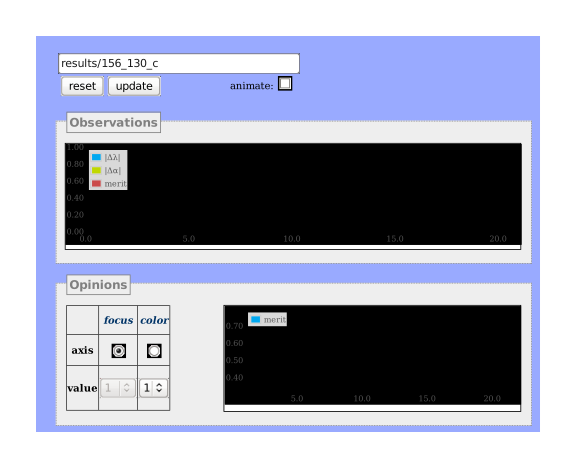
\includegraphics[scale=0.75]{monitor-screenshot.pdf}
\caption{UNCERTIMA Monitor}
\label{fig:monitor-screenshot}
\end{figure}

In the first plot, the expected utility of the currently best
combination (the red curve), and the change rates of the measurement
location (the blue curve) and the best combination (the green curve)
are displayed. When a search algorithm converges, the red curve (the
expected utility) should stabilize around a high value, and the green
curve (the best combination change rate) should approach zero. On the
other hand, the blue curve (the measurement location change rate)
should keep moderate values during most of the algorithm, alternating
betwen relatively low values (exploitation) and high values (exploration).

In the second plot, the belief about the expected utility for each
combination of the parameters can be displayed. The values of all
parameters but the selected one are are fixed in the table on the
left, and the dependency of the belief on the selected parameter for
the chosen values of other parameters is displayed. This plot shows
the user what the search algorithm ``thinks'' about the dependency of
the utility on the parameters at each step of the algorithm, and how
the beliefs are updated. In a future version, a three-dimensional plot
can be used to represent the belief about the expected utility as a
function of two parameters.

\end{document}
